\section{Durchführung}
\label{sec:Durchführung}

\subsection{Bestimmung der Zeitkonstanten}
Zur Bestimmung der Zeitkonstanten $RC$ wird die Schaltung wie in Abbildung \eqref{fig:schaltungzeitkonstante} aufgebaut.
Am Generator wird eine Rechteckspannung eingestellt und die Kondensatorspannung am Oszilloskop beobachtet. Bei passender Einstellung
des Oszilloskops ist die Entladungskurve des Kondensators in Form einer abfallenden Flanke zu sehen.
Von dieser Kurve werden mithilfe des Cursors des Oszilloskops 31 Wertepaare, bestehend aus Kondensatorspannung und Zeit, entnommen. Zuletzt
wird die Kurve als Bild gespeichert.

\begin{figure}[h!]
	\centering
	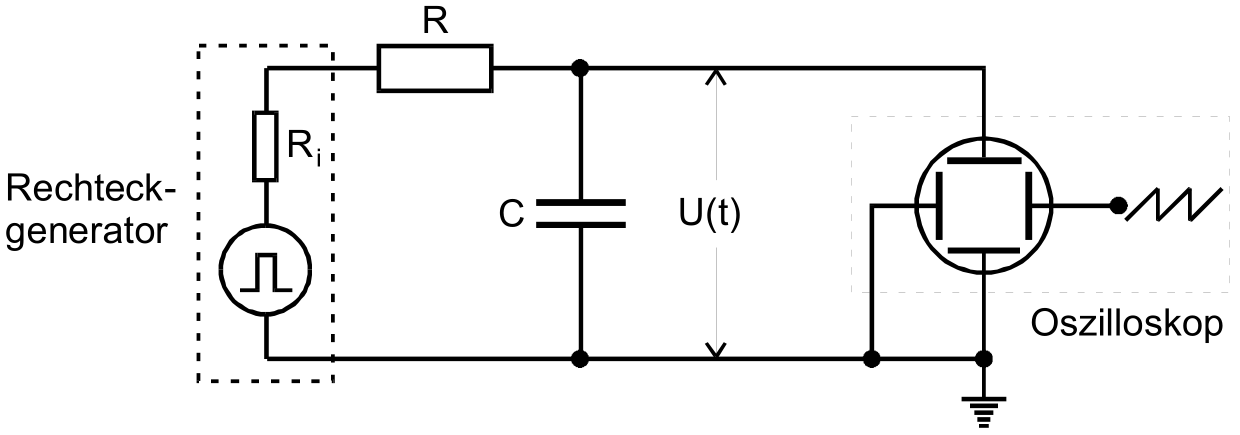
\includegraphics[scale=.45]{content/Schaltung_Zeitkonstante}
	\caption{Messschaltung zur Bestimmung der Zeitkonstanten des RC-Gliedes, \cite[6]{anleitung353}.}
	\label{fig:schaltungzeitkonstante}
\end{figure}


\subsection{Messung der Amplitude in Abhängigkeit von der Frequenz}
In dieser Messung wird der in Abbildung \eqref{fig:schaltungamplitude} zu sehende Aufbau vorgenommen. Nun wird schrittweise die Frequenz am Generator in 
einem Bereich von 10 bis 10000\,Hz erhöht. Für 30 Frequenzen wird die Spannungsamplitude mit dem Cursor gemessen und notiert.

\begin{figure}[h!]
	\centering
	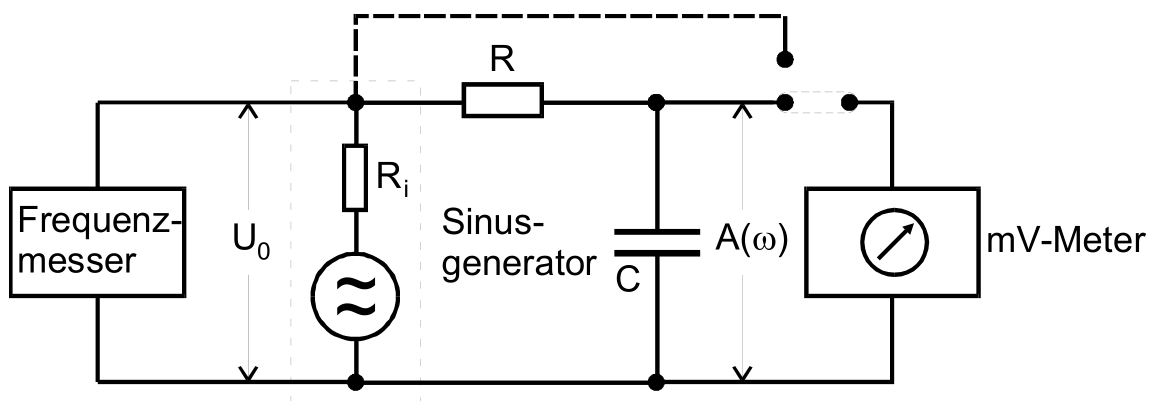
\includegraphics[scale=.45]{content/Schaltung_Amplitude}
	\caption{Messschaltung zur Bestimmung der Amplituden in Abhängigkeit der Frequenz, \cite[7]{anleitung353}.}
	\label{fig:schaltungamplitude}
\end{figure}

\subsection{Messung der Phasenverschiebung in Abhängigkeit von der Frequenz}
Zur Messung der frequenzabhängigen Phasenverschiebung wird die Schaltung wie in Abbildung \eqref{fig:schaltungphasenverschiebung} aufgebaut. 
Am Oszilloskop ist nun die Generator- und die Kondensatorspannung zu sehen. Wie in der zweiten Messung werden nacheinander 22 Frequenzen im Intervall 
von 10 bis 10000\,Hz eingestellt und die Phasenverschiebung der beiden Kurven bestimmt, indem mit dem Cursor der Abstand a gemessen wird 
(vgl. Abbildung \eqref{fig:schaltungphasenverschiebung}). Der Abstand b wird durch Umrechnen der Frequenz zur Periodendauer ermittelt. 

\begin{figure}[h!]
	\centering
	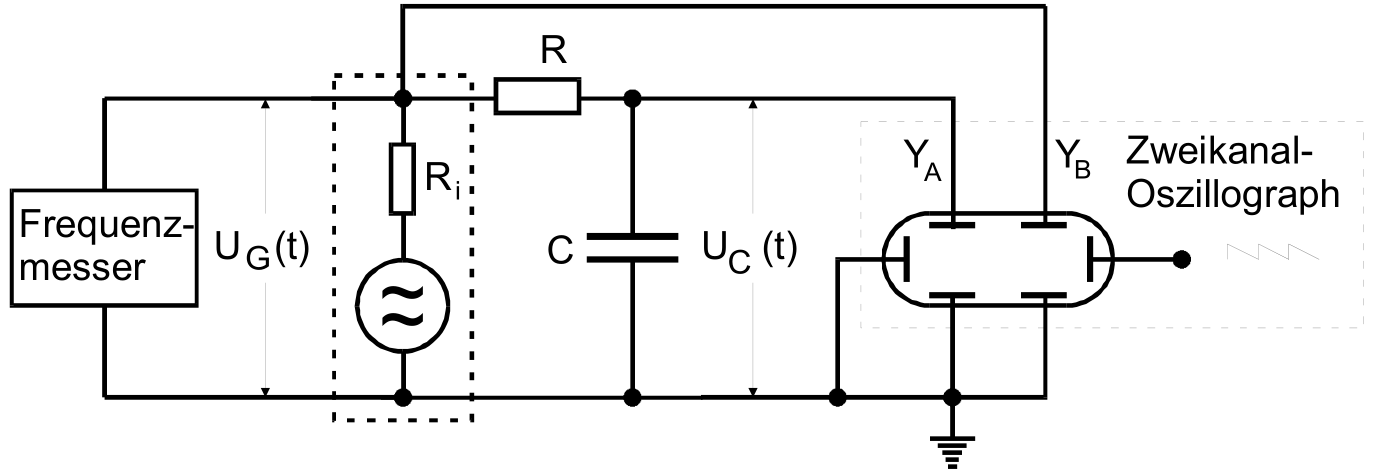
\includegraphics[scale=.45]{content/Schaltung_Phasenverschiebung}
	\caption{Messschaltung zur Bestimmung der Phasenverschiebung in Abhängigkeit der Frequenz, \cite[7]{anleitung353}.}
	\label{fig:schaltungphasenverschiebung}
\end{figure}

\begin{figure}[h!]
	\centering
	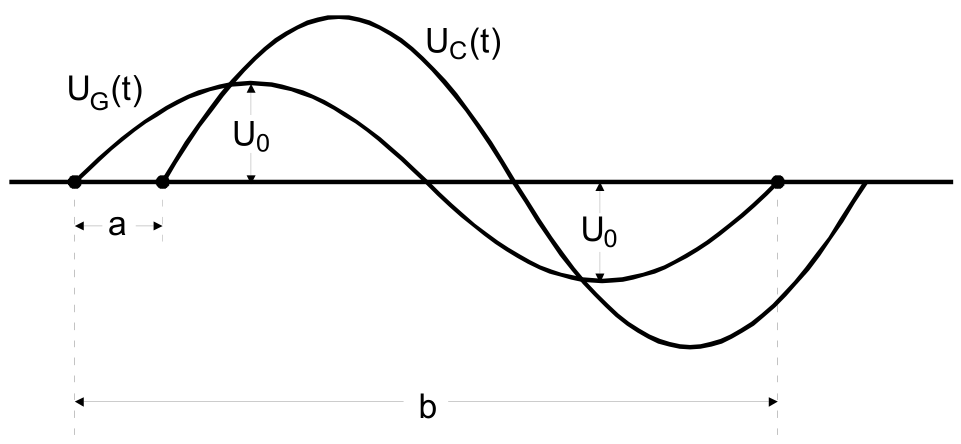
\includegraphics[scale=.55]{content/Abstaende}
	\caption{Messung der Phasenverschiebung zwischen zwei Spannungen, \cite[7]{anleitung353}.}
	\label{fig:abstaende}
\end{figure}

\subsection{RC-Kreis als Integrator}
Um zu zeigen, dass der RC-Kreis als Integrator wirkt, wird die Frequenz der Generatorspannung auf 3000\,Hz gestellt. Anschließend
werden nacheinander Sinus-, Rechteck- und Dreieckspannung an das RC-Glied angelegt. Auf dem Oszilloskop werden nun angelegte und
integrierte Spannung angezeigt, welche dann für jede angelegte Spannung als Bilder gespeichert werden.
